\documentclass{beamer}
\usetheme{Warsaw}
\usecolortheme{wolverine}

\usepackage{xcolor, minted}
\renewcommand\fcolorbox[4][]{\textcolor{cyan}{\strut#4}}
\title{MLIR: Multi-level intermediate representation}
\author{Ramkumar Ramachandra}
\institute{Raincode Labs}
\date{06 December 2022}
\begin{document}
\begin{frame}
  \titlepage
\end{frame}
\begin{frame}{What is MLIR?}
  \begin{columns}
    \begin{column}{3cm}
      
\includegraphics[scale=0.6]{res/mlir-logo}
    \end{column}
    \begin{column}{7cm}
      \begin{itemize}
        \item Compiler infrastructure that factors out work
        \item Multiple \emph{dialects}, with dialect-conversion
        \item Native support for \emph{tensor} and \emph{vector} types
        \item Lowers to the \emph{llvm} dialect, and executes on an LLVM backend
        \item Very young and fast-moving; in LLVM tree
        \item Includes some exciting Polyhedral optimizations
      \end{itemize}
    \end{column}
  \end{columns}
\end{frame}
\begin{frame}{Who uses MLIR?}
  \begin{columns}
    \begin{column}{2cm}
      
\includegraphics[scale=1.0]{res/tf-logo}
      
\includegraphics[scale=0.7]{res/torch-logo}
    \end{column}
    \begin{column}{7cm}
      \begin{itemize}
        \item TensorFlow and an experimental PyTorch backend are the primary users
        \item Various companies are starting to invest in MLIR
        \item Think \emph{quantum} dialect for quantum computing
        \item The \emph{spirv} dialect targets GPUs
      \end{itemize}
    \end{column}
  \end{columns}
\end{frame}
\begin{frame}{An example from the \emph{linalg} dialect}
  \inputminted[linenos, fontsize=\footnotesize]{text}{res/linalg.mlir}
\end{frame}
\begin{frame}{Lowering to the \emph{llvm} dialect}
  \inputminted[linenos, fontsize=\footnotesize]{text}{res/llvm.mlir}
\end{frame}
\begin{frame}
  \begin{itemize}
    \item May optionally use external libraries like cuBLAS, cuDNN, BLAS, MKL
    \item ... and emit C code
    \item There is an \emph{emitc} dialect
  \end{itemize}
\end{frame}
\begin{frame}{Mental model of lowering}
  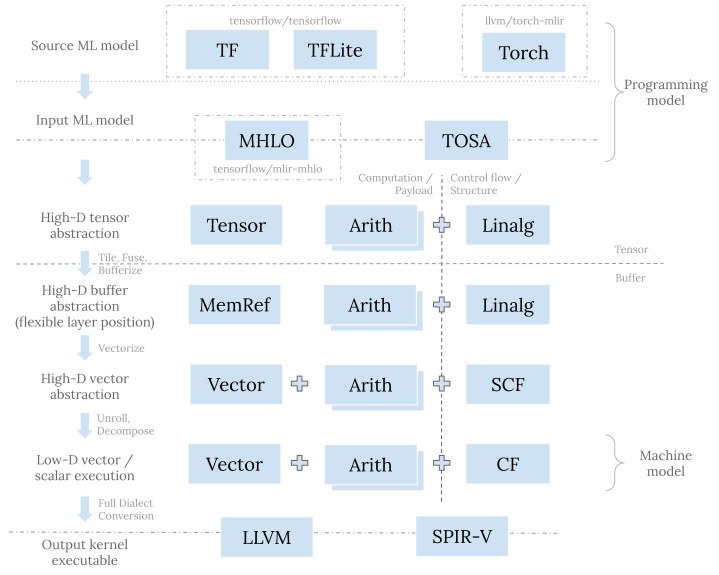
\includegraphics[scale=0.5]{res/lowering}
\end{frame}
\begin{frame}{Is MLIR only suitable for ML-like applications?}
  \begin{itemize}
    \item The joke is that MLIR actually stands for "machine-learning intermediate representation"
    \item More seriously, there are experimental projects compiling C++ and Python to MLIR; Cf. Polygeist and Pylir
    \item The framework is general enough to accommodate any new application
    \item Chris plans to base LLVM on MLIR in the future!
  \end{itemize}
\end{frame}
\begin{frame}{Where to go next}
  \begin{itemize}
    \item mlir.llvm.org
    \item Toy example in tree
    \item Pylir, an AOT Python compiler based on MLIR
    \item No better way to learn than to write your own toy compiler based on MLIR
  \end{itemize}
\end{frame}
\end{document}
